% Appendix Template

\chapter{The Debugger Application} % Main appendix title

\label{Appendix3} % Change X to a consecutive letter; for referencing this appendix elsewhere, use \ref{AppendixX}

\lhead{Appendix 3. \emph{The Debugger Application}} % Change X to a consecutive letter; this is for the header on each page - perhaps a shortened title

As part of the thesis, I have written a Debugger web application to visualize results
and navigate through a loaded trace. This appendix is meant to elaborate on the structure
of the web application. Further details and application code can be found on \url{https://github.com/sankalp-sangle/FlaskDebugger}

The home page of the application provides a recommendation on what could possibly be the cause of fault in the scenario.
\begin{figure}[htbp]
	\centering
		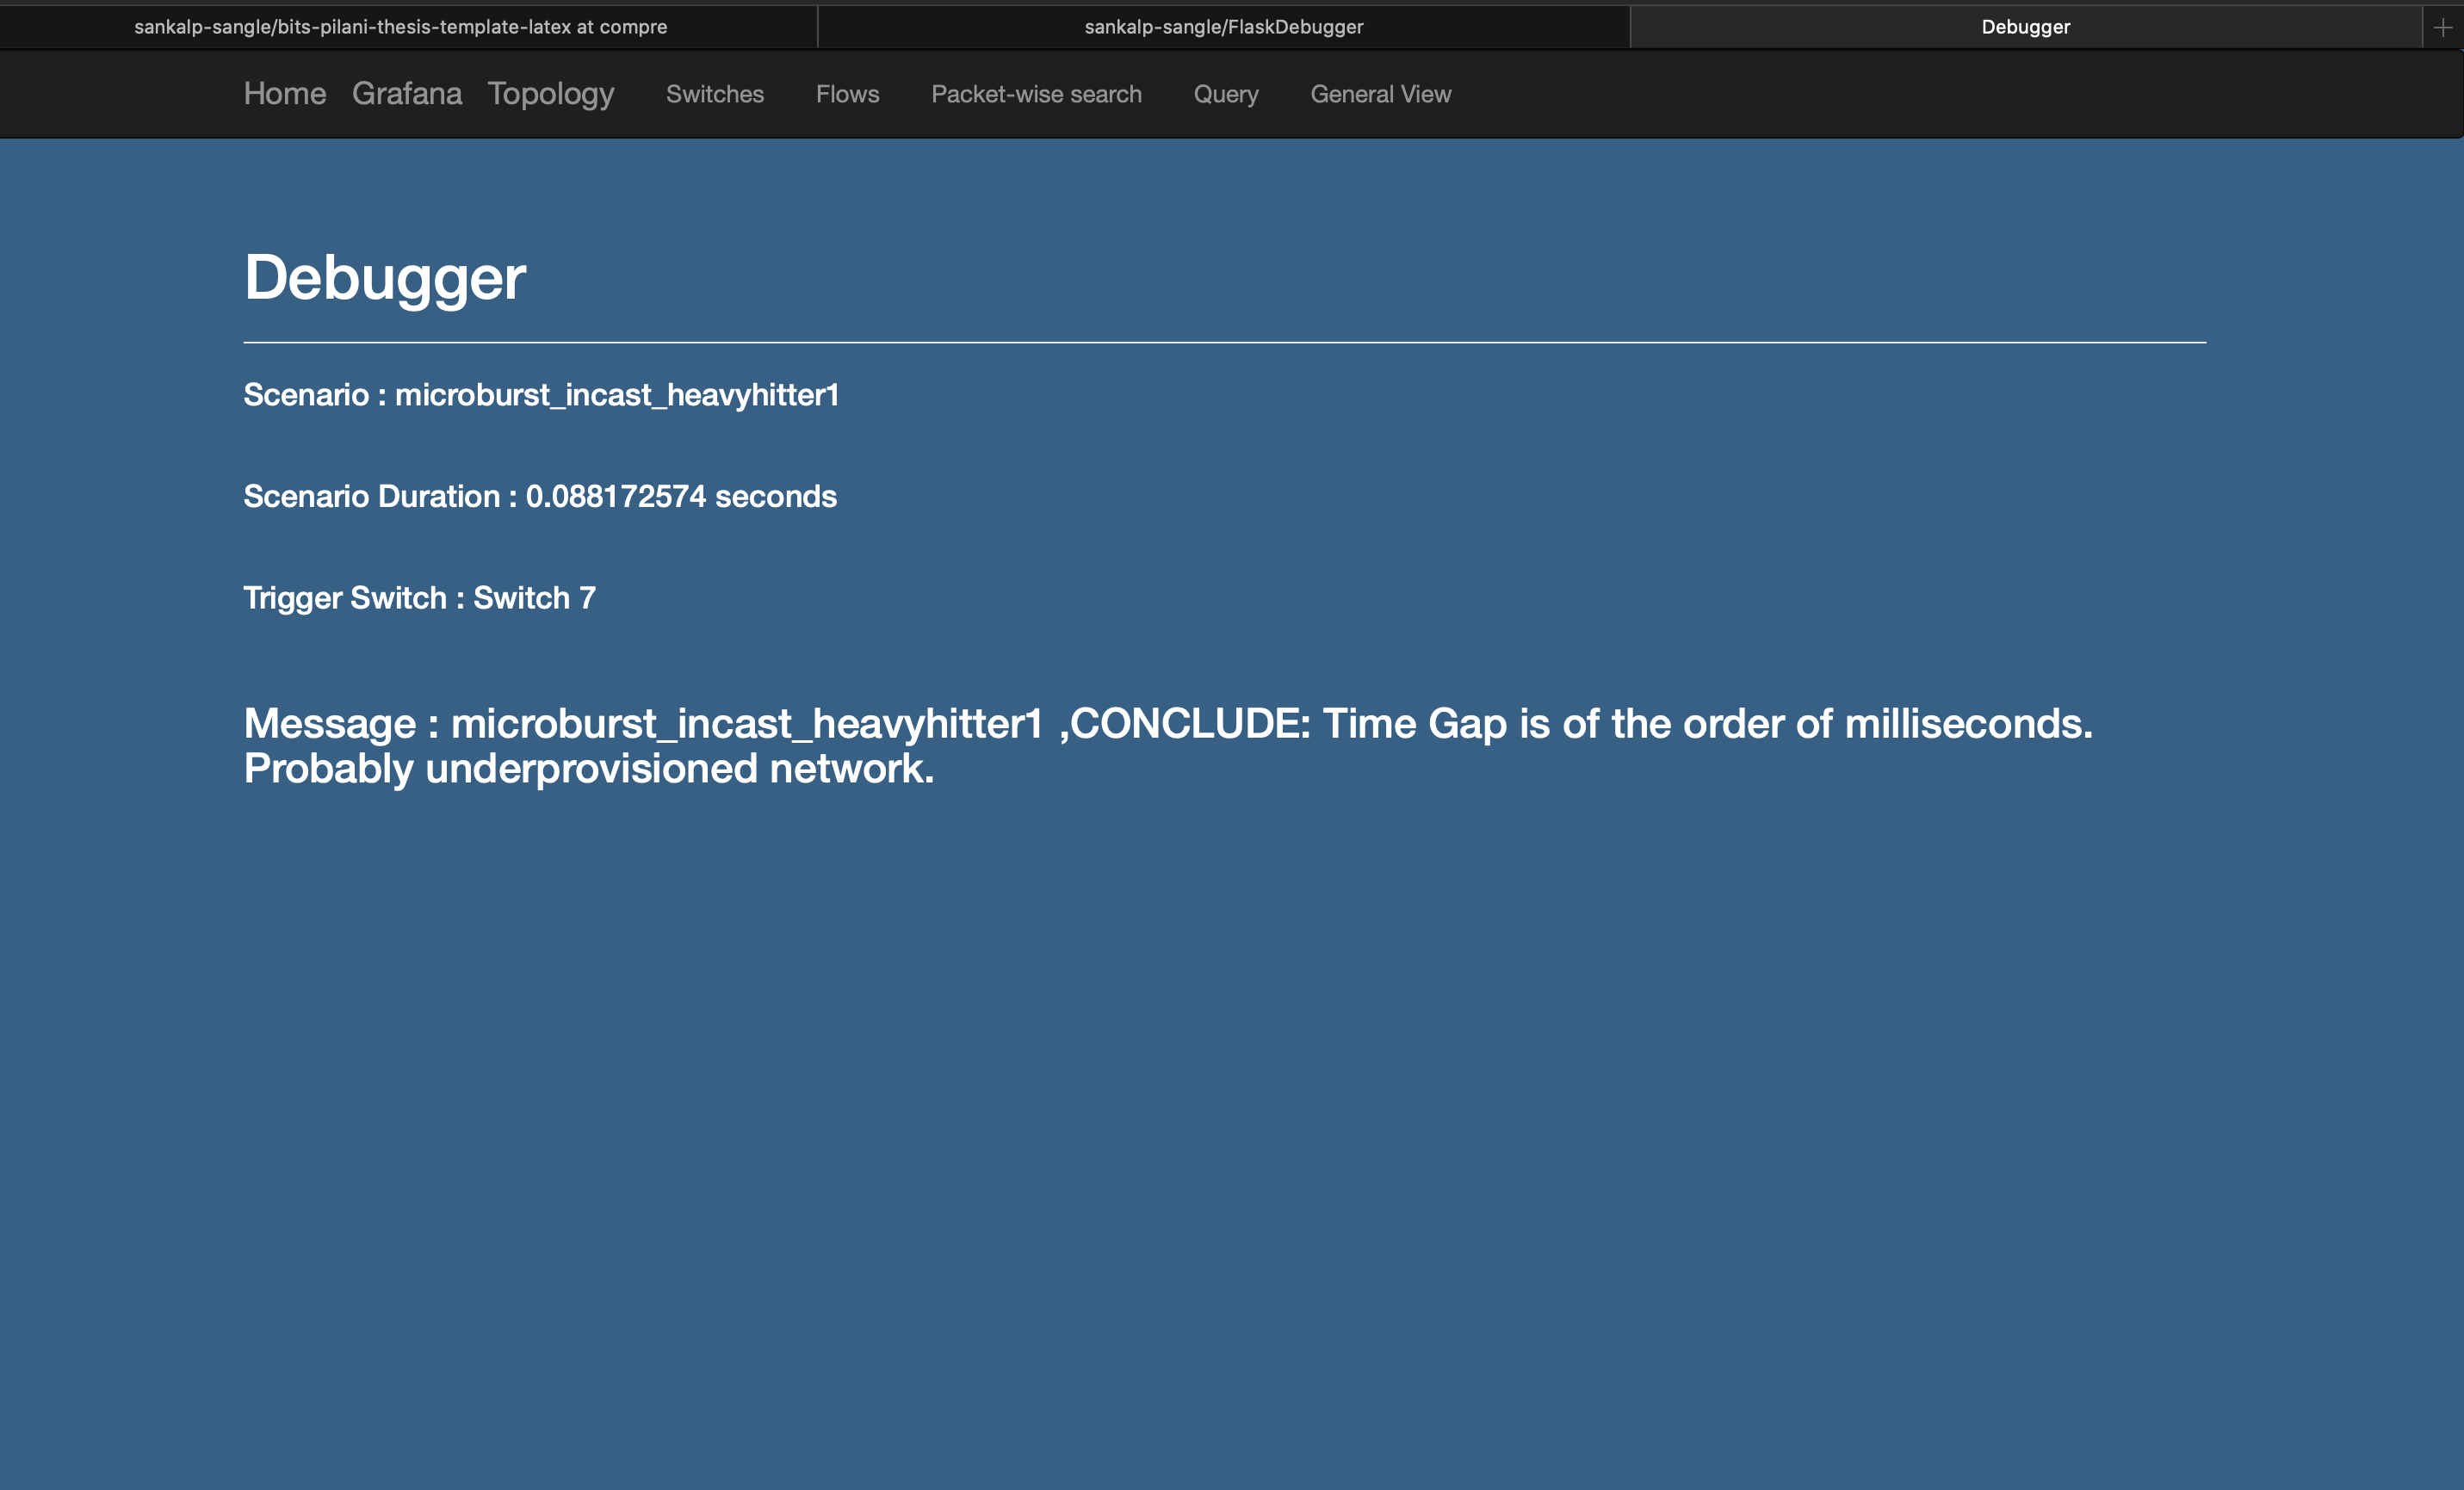
\includegraphics[width=1.0\columnwidth]{Figures/home.png}
		\rule{35em}{0.5pt}
	\caption[Home Page]{Home Page}
	\label{fig:home}
\end{figure}

From the home page, one can navigate to the topology page to view the network topology.
The switches are arranged in order of levels, with switches closer to the core being displayed at the top.
\begin{figure}[htbp]
	\centering
		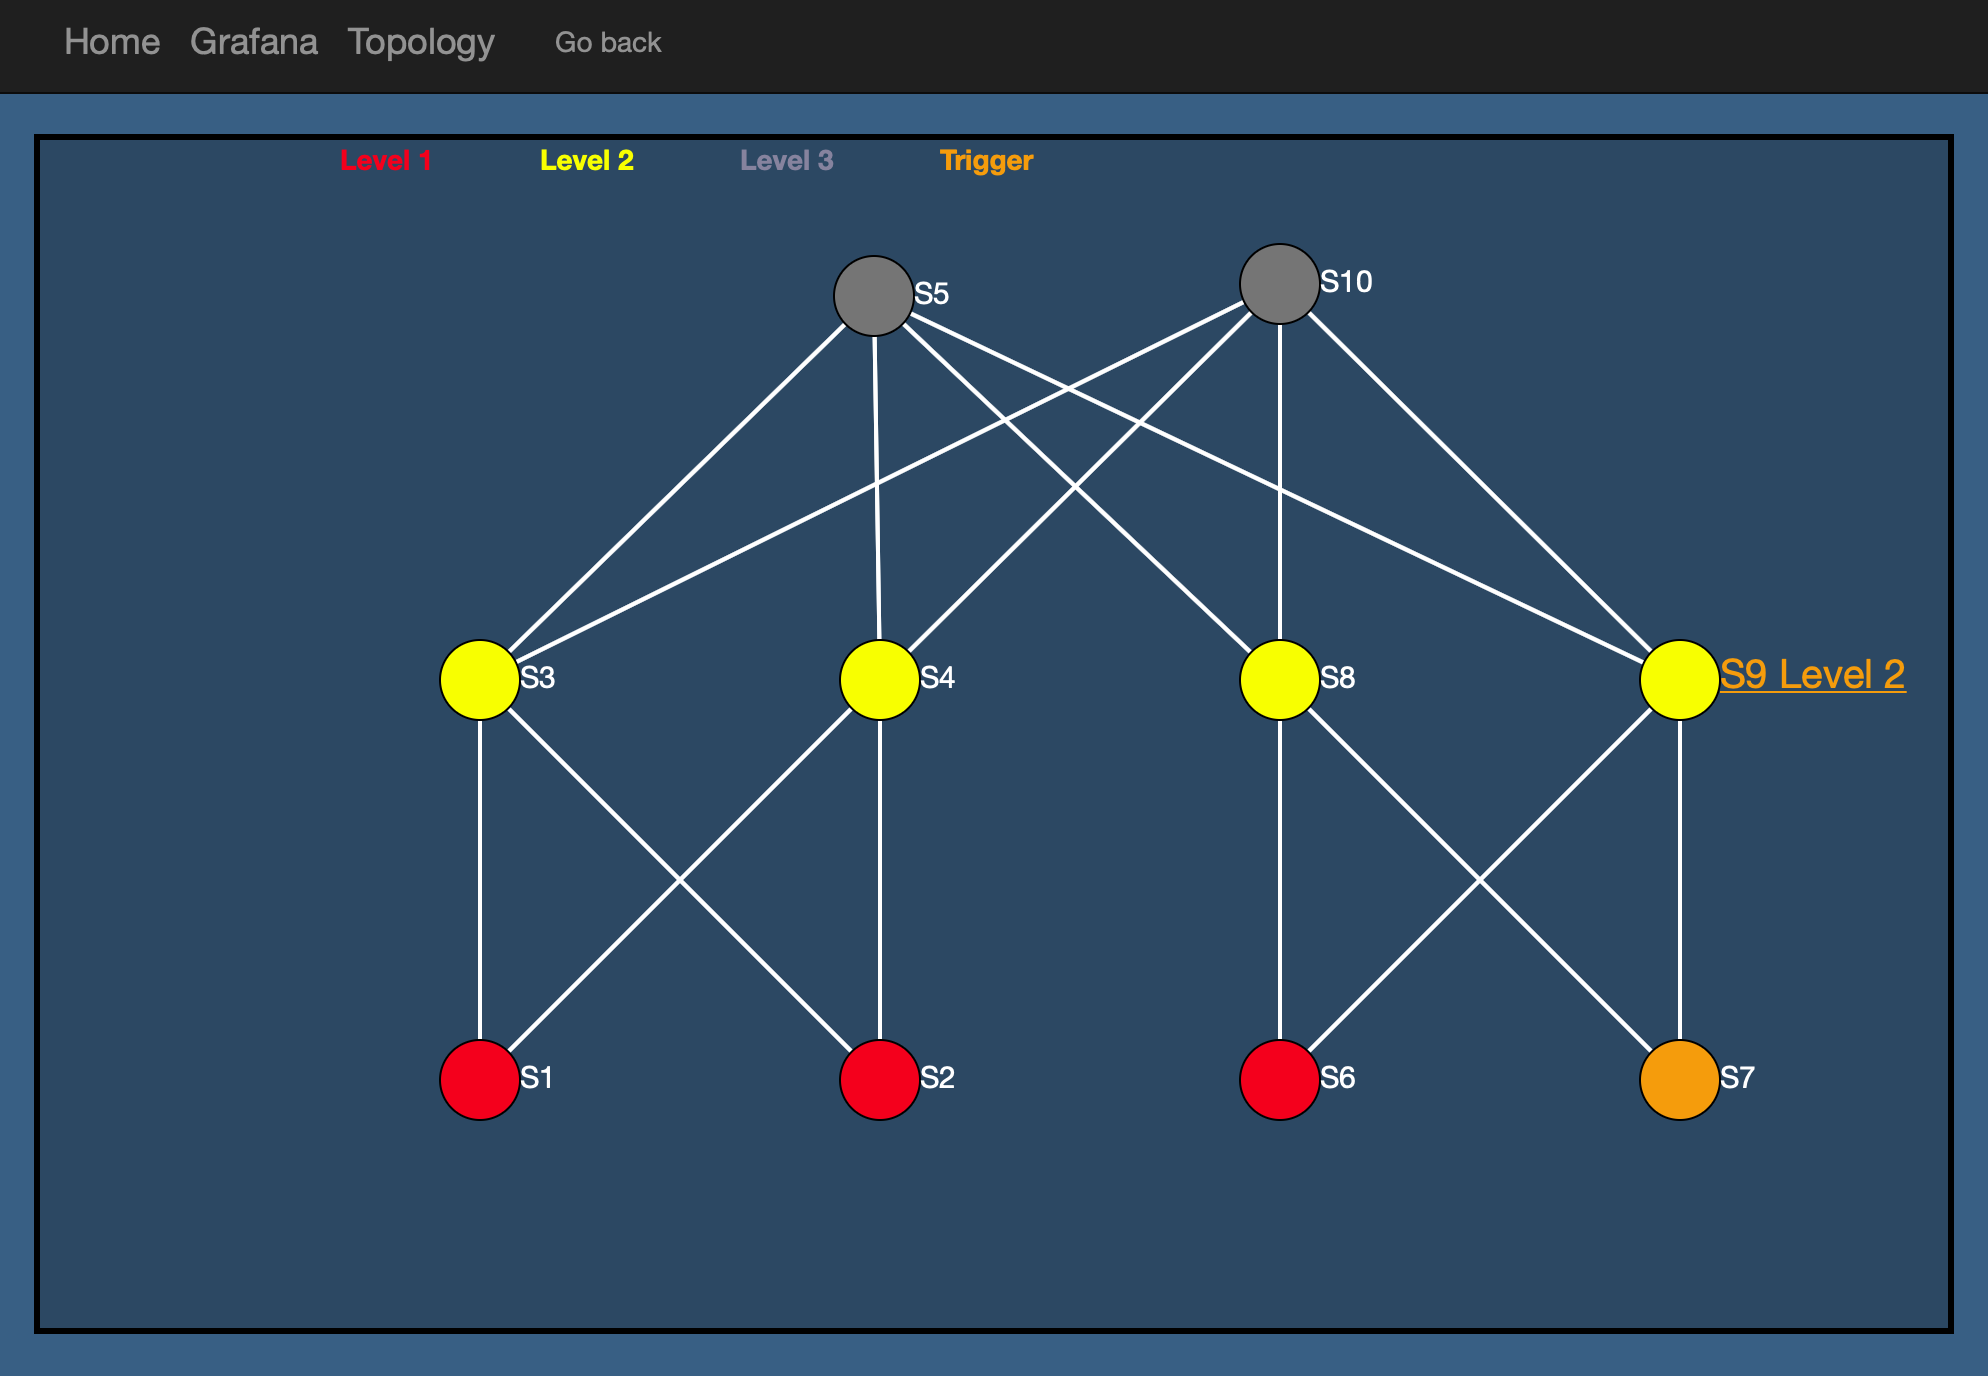
\includegraphics[width=0.85\columnwidth]{Figures/topo.png}
		\rule{35em}{0.5pt}
	\caption[Topology]{Topology}
	\label{fig:topo}
\end{figure}

One can click on any of the switches to see details about that switch.
\begin{figure}[htbp]
	\centering
		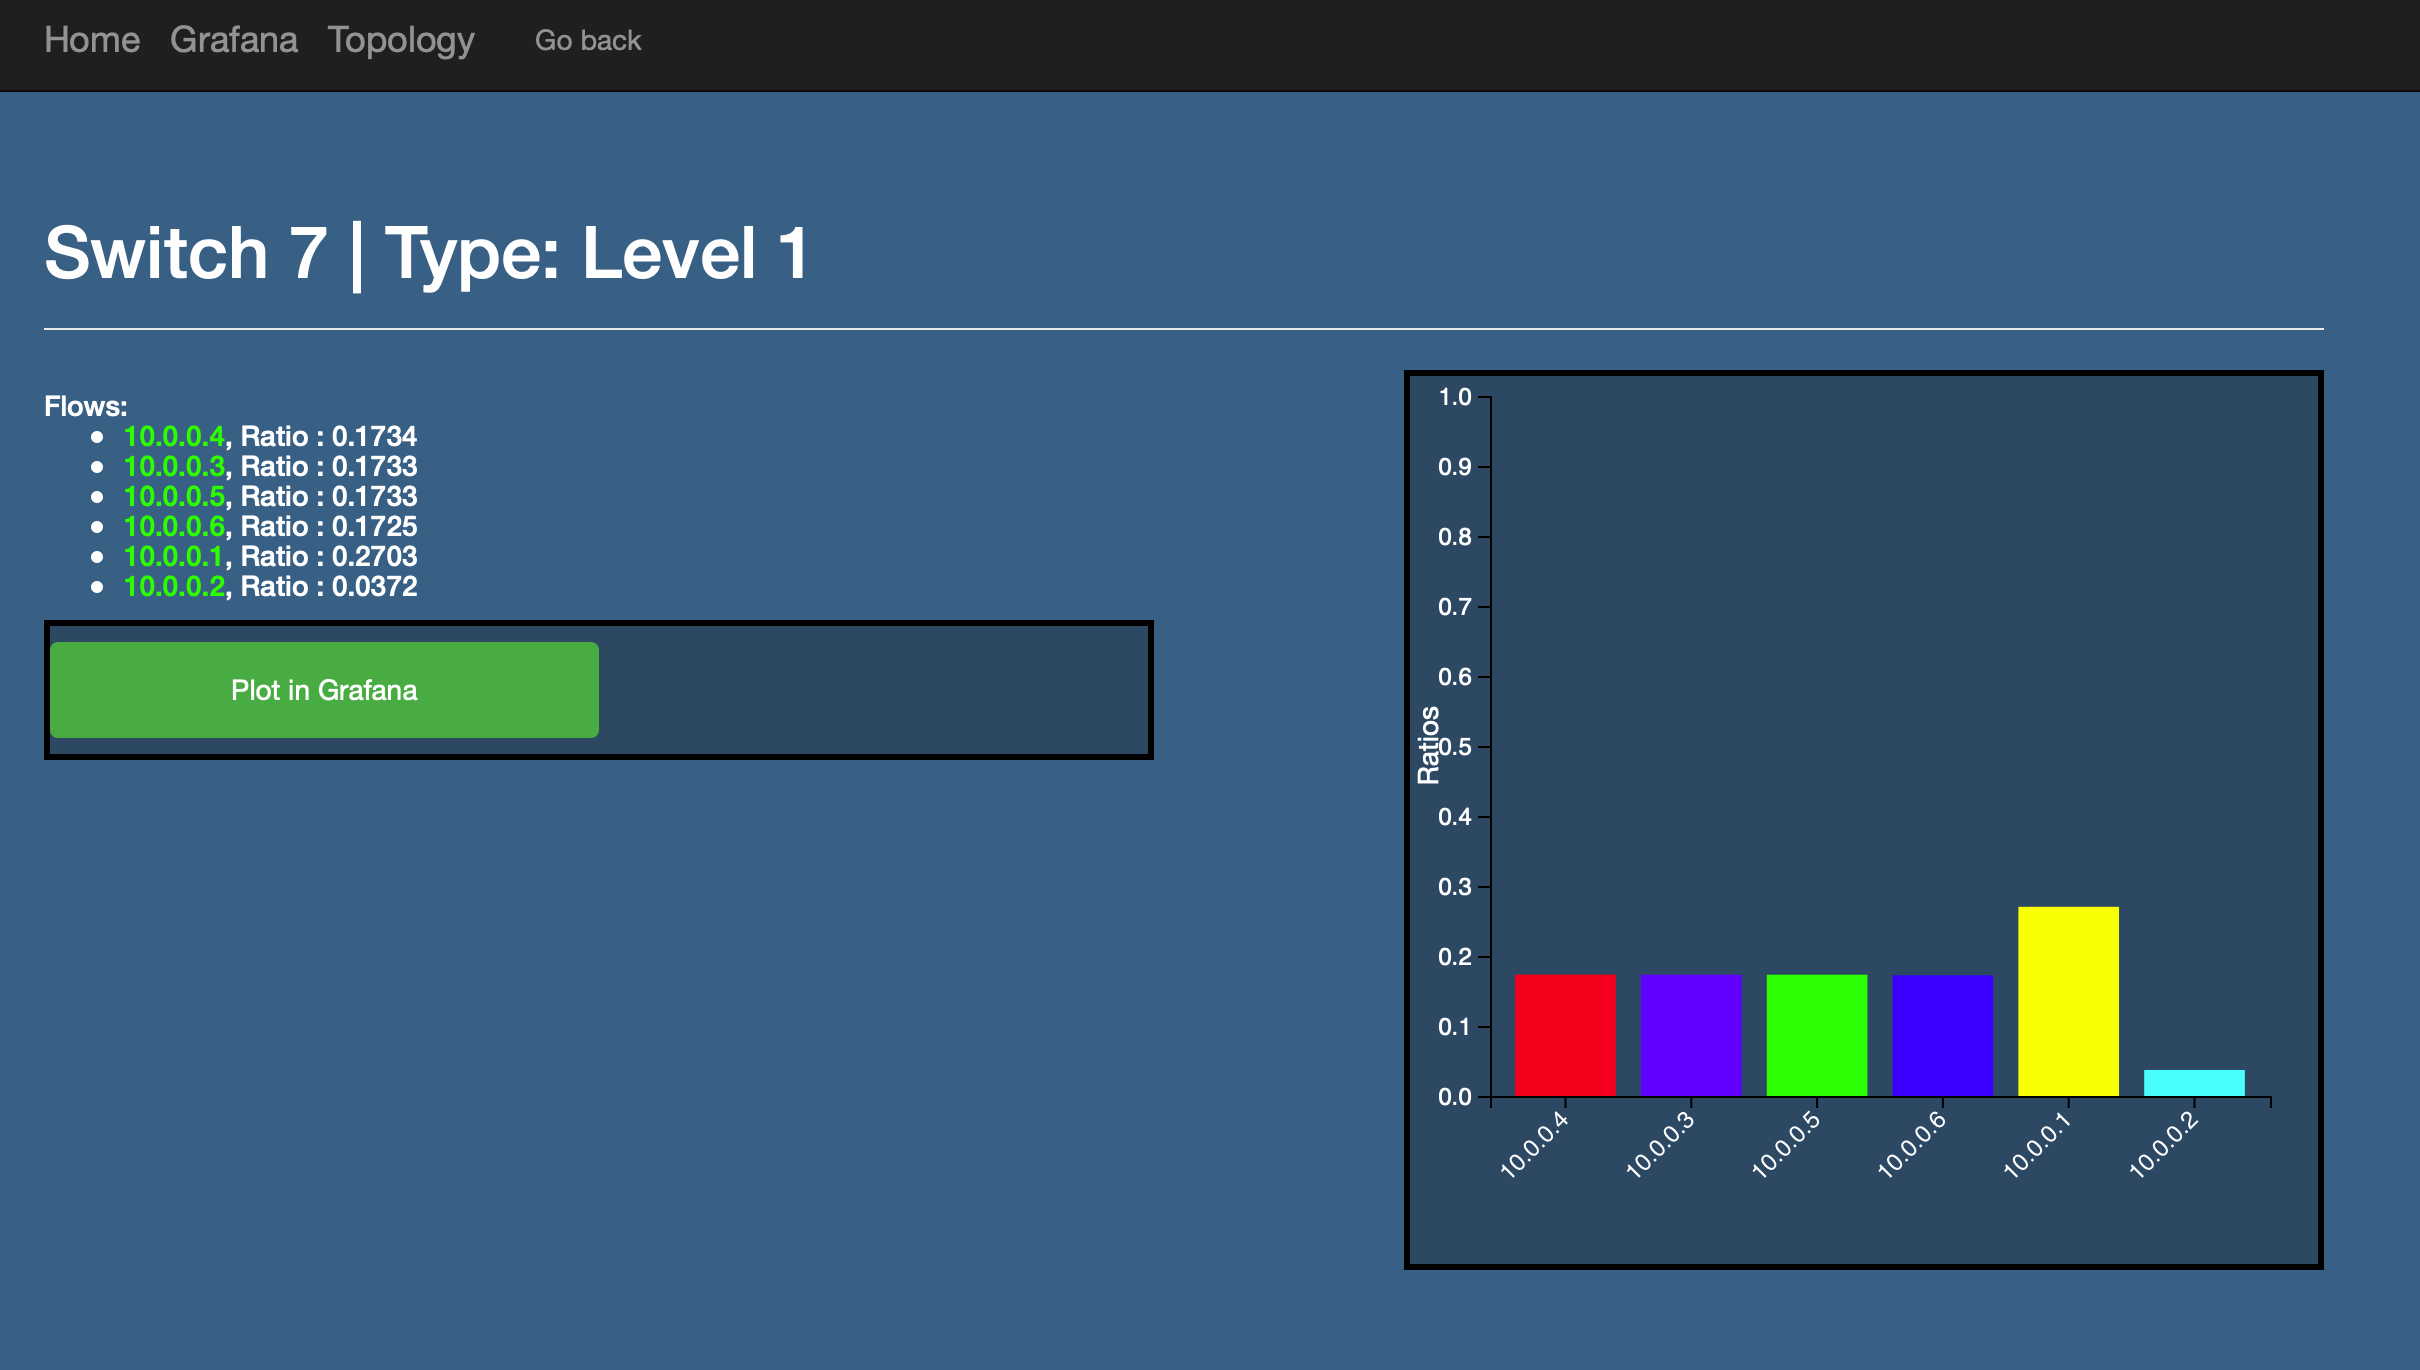
\includegraphics[width=0.85\columnwidth]{Figures/switch.png}
		\rule{35em}{0.5pt}
	\caption[Switch Information]{Information about switch 7}
	\label{fig:switch}
\end{figure}

\newpage

If one wishes to view details about a particular flow, one can click on the
the IP address to view more information such as switches visited.

\begin{figure}[htbp]
	\centering
		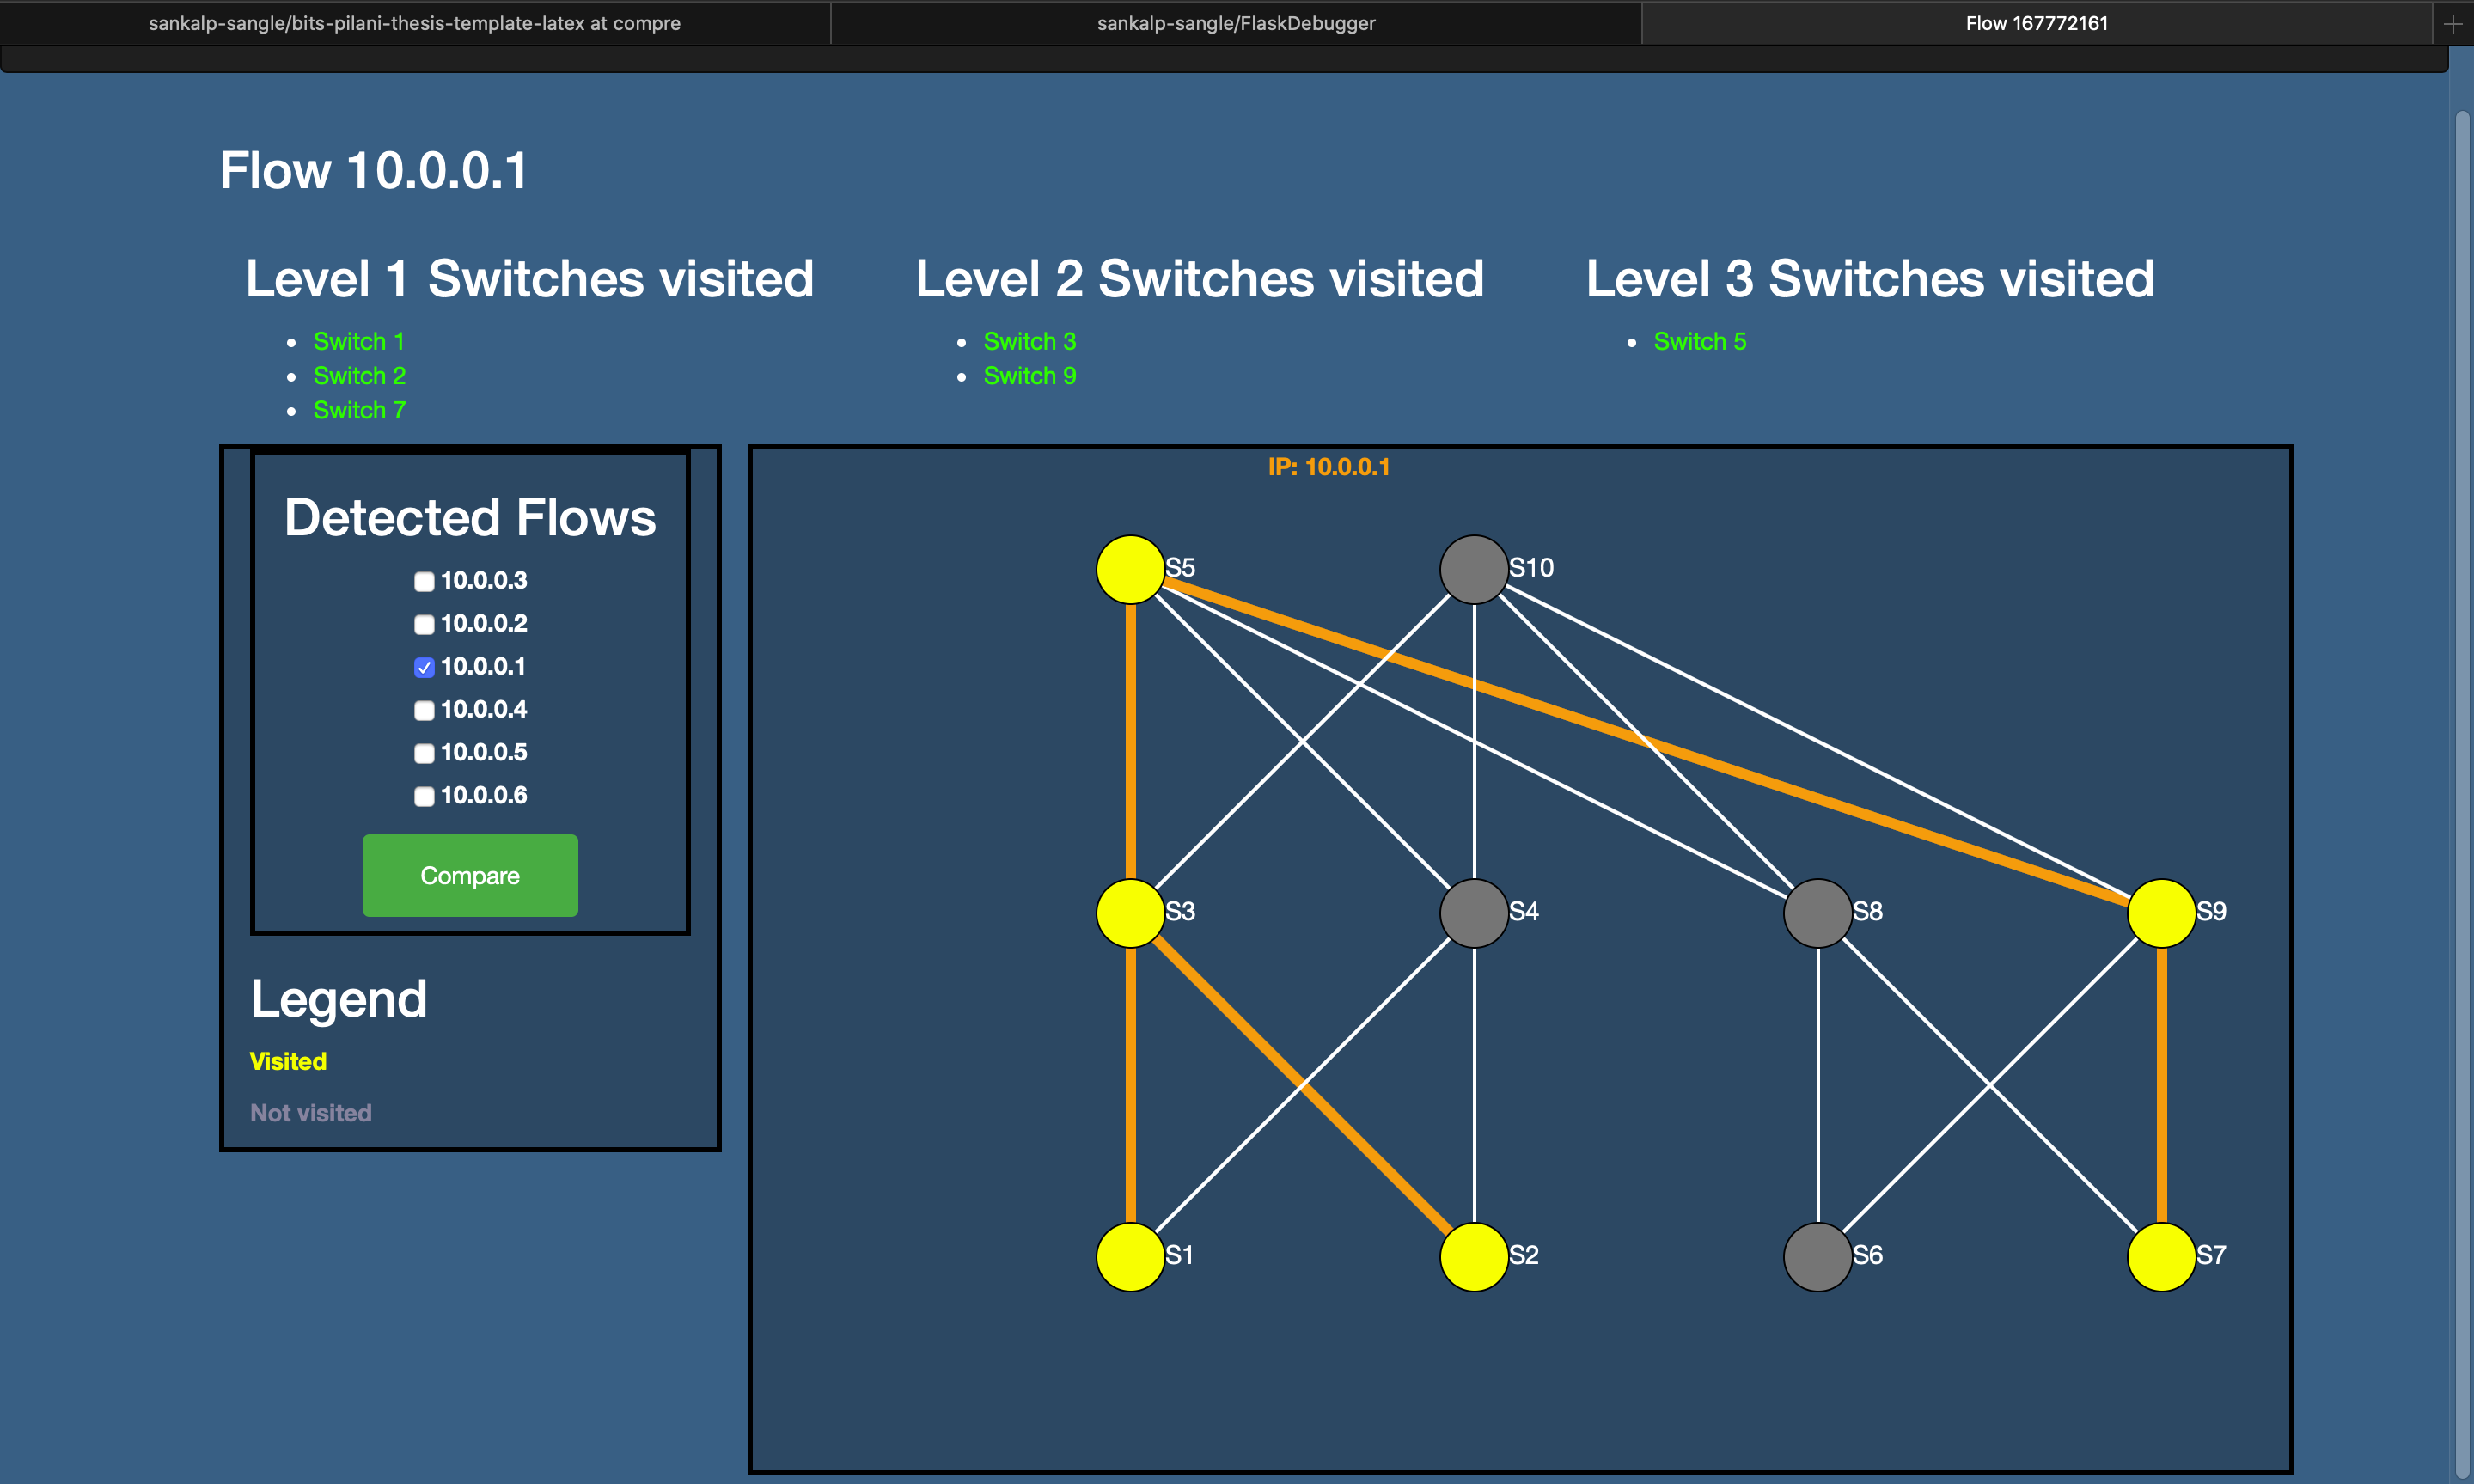
\includegraphics[width=1.0\columnwidth]{Figures/flow.png}
		\rule{35em}{0.5pt}
	\caption[Flow Information]{Flow Information}
	\label{fig:flow}
\end{figure}

Finally, if one wishes to see a birds eye view of the topology and replay it back, one can
do so via the General View tab. We have options to pause, play, speed up and slow down the playback.

\begin{figure}[htbp]
	\centering
		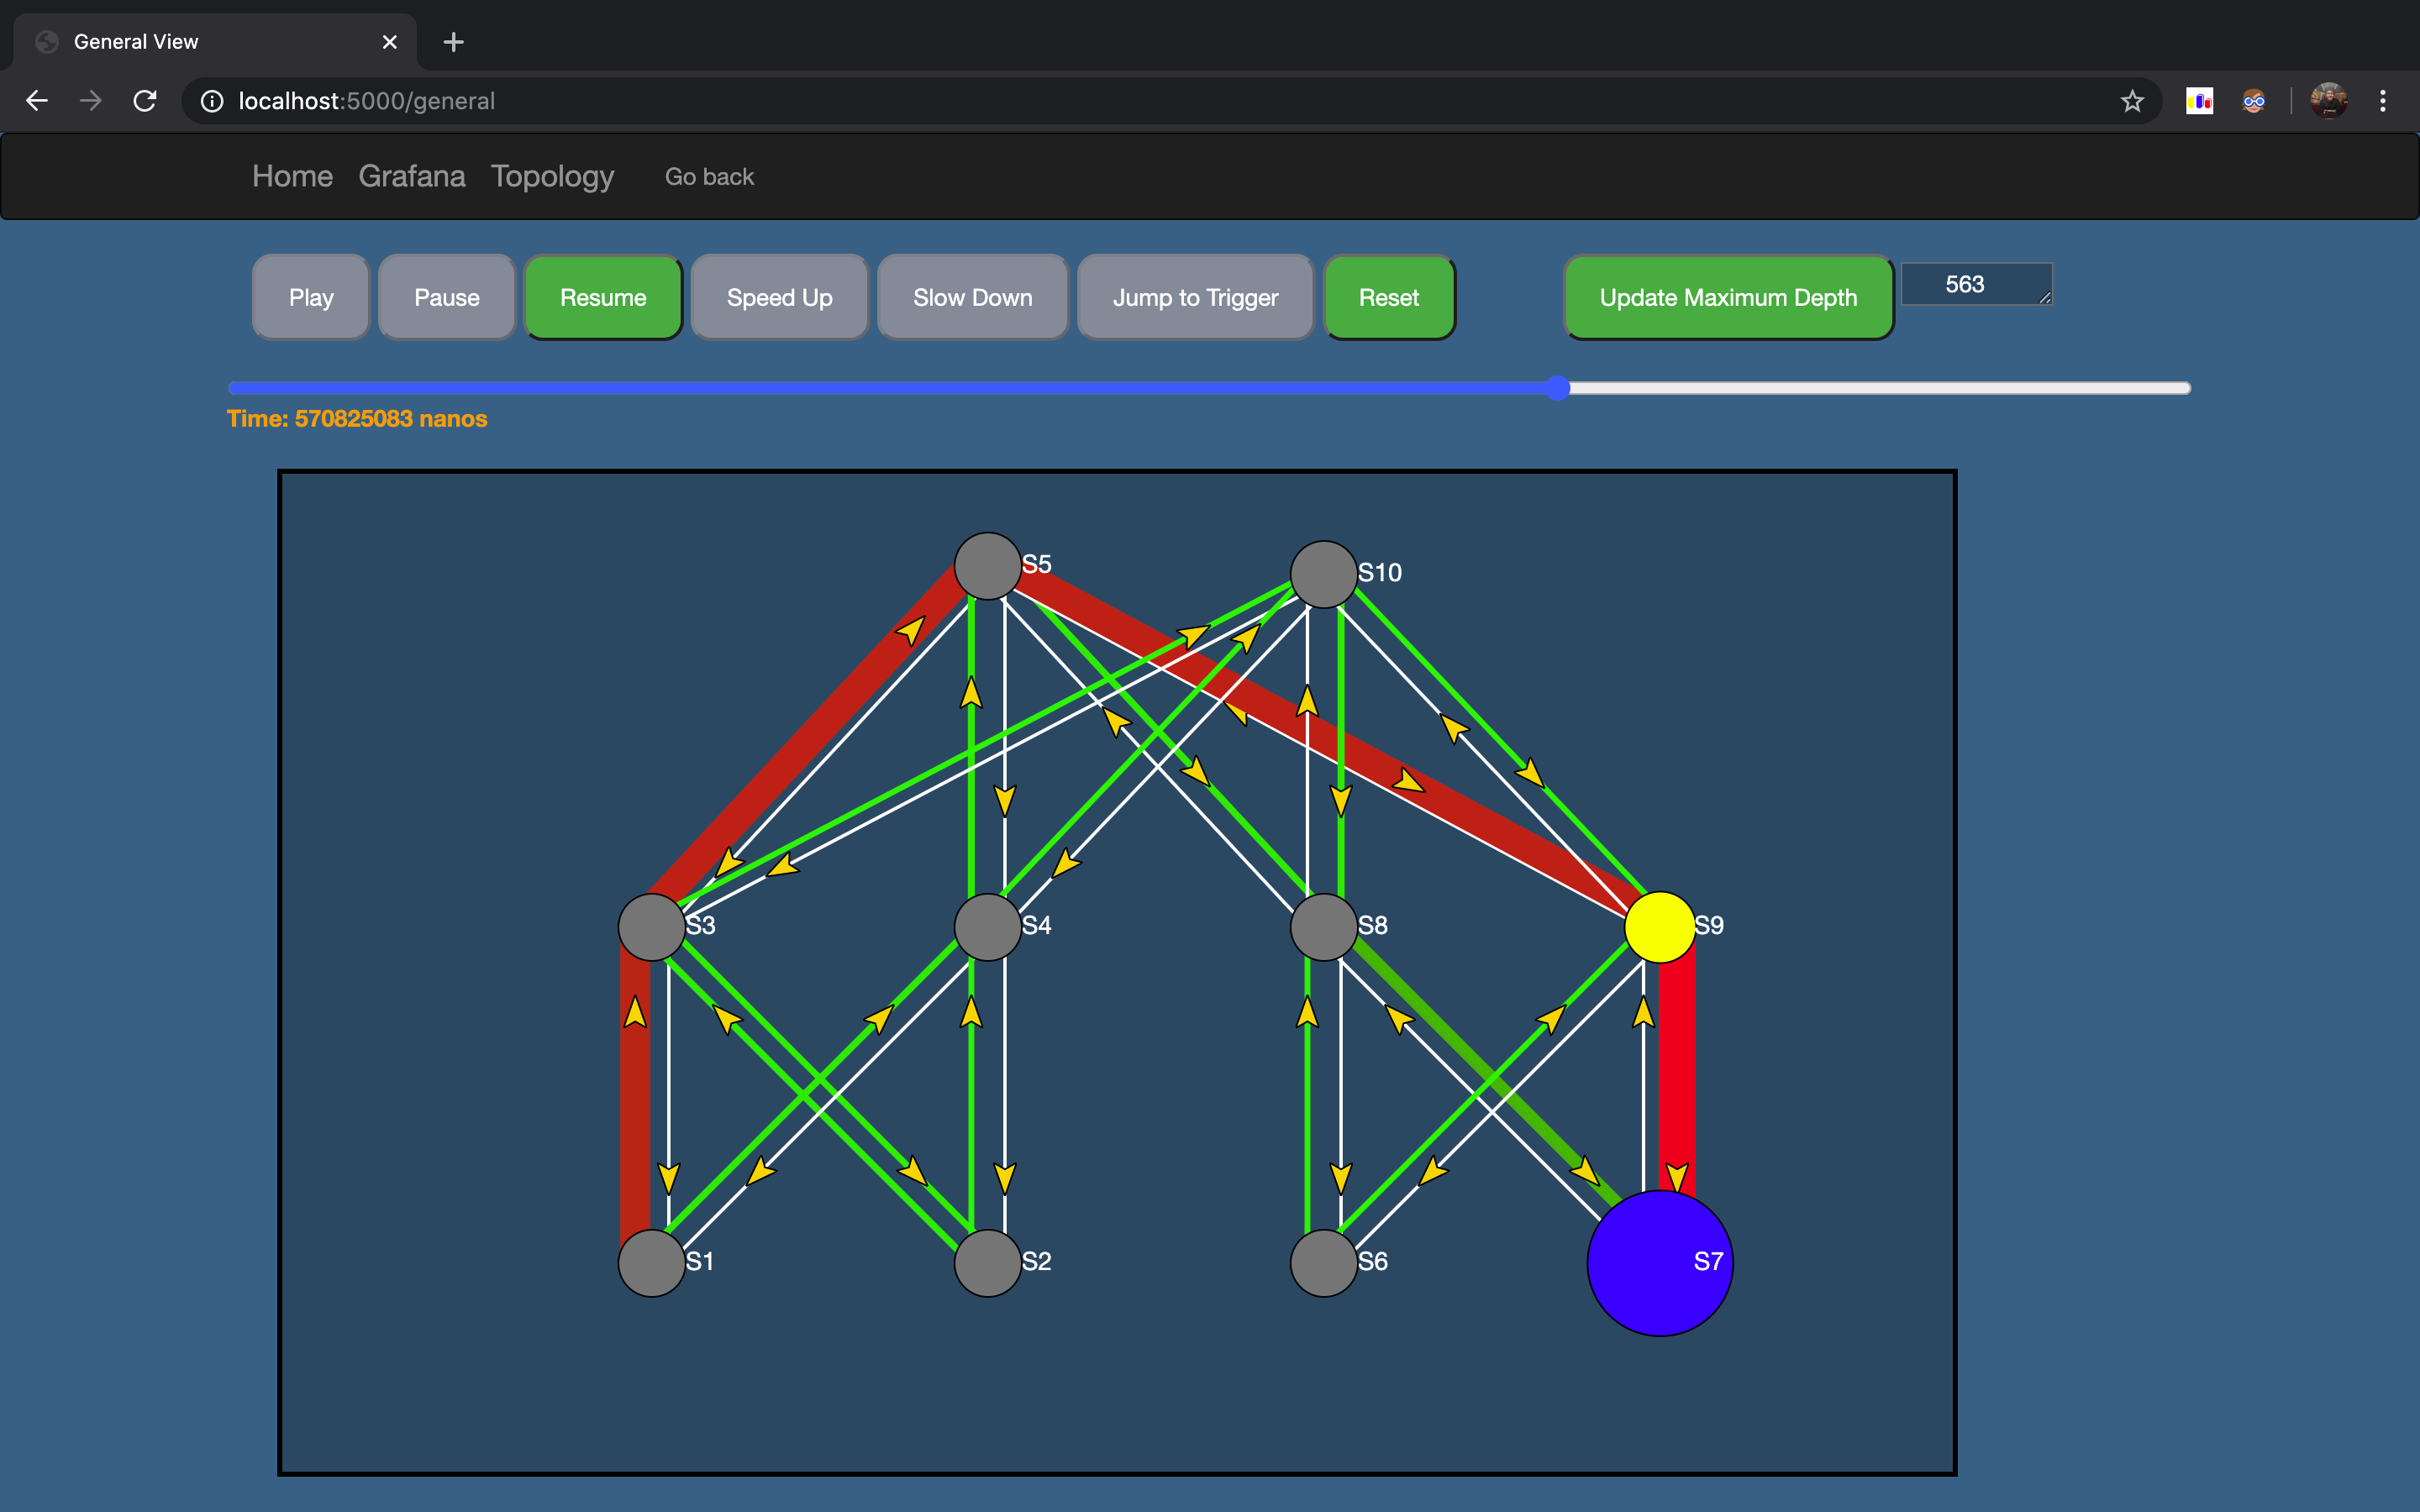
\includegraphics[width=1.0\columnwidth]{Figures/genview.png}
		\rule{35em}{0.5pt}
	\caption[Birds eye view]{A birds eye view of the scenario}
	\label{fig:birdseye}
\end{figure}